%\documentclass[10pt,a4paper,twocolumn]{article}
\documentclass[10pt,a4paper]{article}
\usepackage[utf8]{inputenc}
\usepackage{amsmath}
\usepackage{amsfonts}
\usepackage{amssymb}
\usepackage{graphicx} 
\usepackage{subfigure}
\usepackage{paralist}
\usepackage{hyperref}
\usepackage{comment} %for anonymized version everything removed for anonymization is in \excludecomment{}

\usepackage{hyperref,xcolor}
%\usepackage{algpseudocode}
\usepackage[lined,boxed]{algorithm2e}
\usepackage[english]{babel}
\usepackage{graphicx}
\usepackage{url}
\usepackage{geometry}
\usepackage{mathrsfs}
\usepackage{color}
\usepackage{sidecap}
\usepackage{bbold}
\usepackage{caption}

\usepackage{ gensymb } % for \degree
\usepackage{ amssymb } % for \varnothing

\definecolor{canard}{rgb}{0,0.4,0.2}
\definecolor{wine}{rgb}{0.4,0,0.2}
\definecolor{marron}{rgb}{0.9,0.4,0.1}
\hypersetup{
  colorlinks,
  linkcolor=canard
}

%\definecolor{canard}{rgb}{1,0,1}
%\definecolor{canard}{rgb}{0,1,1}



\DeclareMathOperator*{\argmin}{\arg\!\min}
\DeclareMathOperator*{\argmax}{\arg\!\max}

\geometry{left=3.5cm , right=3cm}


\usepackage{url}
\usepackage{booktabs}

\usepackage{tikz}
\usetikzlibrary{arrows, decorations.markings}
\usetikzlibrary{fit}
\usetikzlibrary{positioning, calc}

\usepackage[draft,nomargin,footnote]{fixme}

\graphicspath{{figs/}}

\usepackage{xspace}
\newcommand{\eg}{\textit{e.g.}\xspace}
\newcommand{\etal}{\textit{et al.}\xspace}
\newcommand{\ie}{\textit{i.e.}\xspace}
\newcommand{\etc}{\textit{etc.}\xspace}
\newcommand{\vs}{\textit{vs.}\xspace}

\newcommand\given[1][]{\:#1\vert\:}

\begin{document}


\title{Mutual Understanding in Human-Robot Interaction}


%\author{\# \# \#}
\author{Alexis Jacq$^{1,2}$\\
$^1$CHILI Lab, \'Ecole Polytechnique F\'ed\'erale de Lausanne, Switzerland,\\
$^2$Instituto Superior T\'{e}cnico, University of Lisbon, Portugal}



\maketitle
\begin{abstract}
In every collaborative social interaction, agents must be able to understand each other. This mutual understanding requires the ability to establish a mental model of the other, called mutual modelling. 
My \textit{Ph.D.} is focused on mutual modelling in robotics: How robots can model other agents within social activities? Such models must be dynamic in order to keep track of shared knowledge, and adaptive in order to deal with specific behaviours of agents. We introduce a new approach to implement second-order of modelling in order to maintain a mutual understanding between human and robot. 
%We ask the question: Would an architecture able of second-order modelling improve Human-Robot Interactions ?
This work is directly applied to the CoWriter Project, that aims at exploring how a robot can help children with the acquisition of handwriting~\footnote{http://chili.epfl.ch/cowriter}. 
In this context, would a robot able of second-order of mutual modelling improve this educative Child-Robot-Interaction?
\end{abstract}
%\newpage

%\tableofcontents

\section{Introduction}
\subsection{Importance of higher levels of Mutual Modelling in HRI}
A social robot is required to interact with humans. 
The quality of this interaction depends on its ability to behave in an acceptable and understandable manner by the user. 
Hence it is important for the robot to take care of its image: how much it is perceived as an automatic and repetitive agent, or contrarily as a surprising and intelligent character. If the robot is able to detect this perception of itself, it can adapt its behaviour in order to be understood: ``\textit{you think I am sad while I am happy, I want you to understand that I am happy}". 

In a collaborative context, where knowledge must be shared, agents must exhibit that they are acquiring the shared information with an immediate behaviour: ``\textit{I look at what you are showing me, do you see that I am looking at it, do you think I am paying attention to your explanation ?}"; ``\textit{I have understood your idea, do you understand that I have understood ?}". 
As humans, we have different strategies to exhibit understanding or to resolve a misunderstanding. 
As an example, if someone is talking about a visual object, we alternatively gaze between the object and the person to make sure he saw that we gazed at the object. Or if we detect that the other person has not understood a gesture (e.g. pointing at an object) we would probably exaggerate the gesture.

Developed by Baron-Cohen and Leslie~\cite{baron1985does}, the Theory of Mind (ToM) describes the ability to attribute mental states and knowledge to others. In interaction, humans are permanently collecting and analysing huge quantity of information to stay aware of emotions, goals and understandings of their fellows. In this work, we focus on a generalization of this notion: Mutual Modelling characterizes the effort of one agent to model the mental state of another one~\cite{dillenbourg1999you}. 

Until now, the work conduced by the Human-Robot Interaction (HRI) community to develop mutual modelling abilities in robots was limited to a first level of modelling (see related work in section~\ref{rw}). Higher levels require the ability to recursively attribute a theory of mind to other agents (\textit{I think that you think that} ...) and their application to HRI remains unexplored. However, a knowledge of oneself perceived by others is necessary to adapt a behaviour to keep mutual understanding. 

We introduce a framework for mutual modelling in HRI in section~\ref{framework} and present an  architectural approach that enables 1st and 2nd order of mutual modelling and uses models to maintain mutual understanding (see section~\ref{arch}).
Our research question is: \textit{does a second level of modelling enables higher quality interactions?}. 
Section ~\ref{eval} gives details on the operationalization and on the evaluation of our proposed approach.

\subsection{Application to the CoWriter project}
An important challenge of social robotics is to provide assistance in education. 
The ability of robots to support adaptive and repetitive tasks can be valuable in a learning interaction.
The CoWriter Project~\cite{Hood,jacq2016building} introduces a new approach to help children with difficulties in learning handwriting. 
Based on the \emph{learning by teaching} paradigm, the goal of the project is not only to help children with their handwriting, but mainly to improve their self-confidence and motivation in practising such exercise.

\emph{Learning by teaching} engages students to conduct the activity in the role of the teachers in order to support their learning process. 
This  paradigm is known to produce motivational, meta-cognitive and educational benefits in a range of disciplines~\cite{Rohrbeck2003}. 
The CoWriter project is the first application of the learning by teaching approach to handwriting.

The effectiveness of this learning by teaching activity is built on the ``prot\'eg\'e effect'': the teacher feels responsible for his student, commits to the student's success and possibly experiences student's failure as his own failure to teach. 
The main idea is to promote the child's extrinsic motivation to write letters (he does it in order to help his ``prot\'eg\'e" robot) and to reinforce the self-esteem of the child (he plays the teacher and the robot actually progresses).

In that context, the robot needs to pretend enough difficulties to motivate the child to help it. 
This ability of the robot to pretend strongly depends on the perception of the robot by the child: the displayed behaviours (gestures, gazes and sounds) by the robot, the initial level and learning speed of the robot must match with what the child imagines of a ``robot in difficulty".
In order to adapt to the child, the robot needs then to have a model of how it is perceived by the child. On the other side, the child builds also a model of the robot's difficulties and attitude. 
This mutual-modelling is primordial in order to have mutual understanding and fluid interaction between learner and teacher. 

The section~\ref{year} shows all my contributions to this project, and explain how those contributions have prepared the ground for incoming studies and define the starting point for experimental verifications of the importance of our mutual modelling approach.
%todo decri bien le fait je vais presenter 3 expe et après je voues explique en quoi elles nous on aider pour notre travail de MM
\section{Related work}\label{rw}


In various fields, frameworks were proposed in order to describe the mutual modelling ability~\cite{lemaignan2015mutual}. 
In developmental psychology Flavell~\cite{flavell1990developmental} denotes two different levels of perspective taking: the \textit{cognitive connection} (I see, I hear, I want, I like...) and \textit{mental representation} (what other agents feel, hear, want...).

From a computational perspective, Epistemic logic describes knowledges and beliefs shared by agents. This framework enables consideration of infinite-level of mutual modelling. It defines a \textit{shared-knowledge} (all the agents of a group know \textbf{X}) and a \textit{common-knowledge} (all the agents of a group know \textbf{X}, and know that all the agent know \textbf{X}, and know that all the agents know that all the agents know \textbf{X}, \dots.)~\cite{hendricks2008epistemic}. 

Mutual modelling has also been studied through educational contexts. Roschelle and Teasley~\cite{roschelle1995construction} suggested that collaborative learning requires a \textit{shared understanding} of the task and of the shared information to solve it. 
The term ``mutual modelling" was introduced in Computer-Supported Collaborative Learning (CSCL) by Dillenbourg~\cite{dillenbourg1999you}. It focused on knowledge states of agents. Dillenbourg developed in \cite{sangin2007partner} a computational framework to represent mutual modelling situations.

However, HRI research has not, until now, explored the whole potential of mutual modelling. In \cite{scassellati2002theory}, Scassellati supported the importance of Leslie's and Baron-Cohen's theory of mind to be implemented as an ability for robots. 
He focused his work on attention and perceptual processes (face detection or colour saliency detection). Thereafter, some works (including Breazeal~\cite{breazeal2006using}, Trafton~\cite{Trafton2005}, Ros~\cite{Ros2010} and Lemaignan~\cite{lemaignan2012thesis}) were conduced to implement Flavell's first level of perspective taking~\cite{flavell1977development} (``\textit{I see (you do not see the book)}"), ability that is still limited to visual perception. 

Breazeal~\cite{breazeal2009embodied} and Warnier~\cite{warnier2012when} reproduced the Sally and Anne's test of Wimmer~\cite{wimmer1983beliefs} with robots able to perform visual perspective taking. The robot was able to infer the knowledge of a human given the history of his visual experience.



\section{Development \& experiments with CoWriter}\label{year}
During the first year of my \textit{Ph.D.} I worked on the development of the CoWriter activity. 
I improved the content of the interaction: proposed an algorithm to learn and generate letters, generated automatic behaviours for the robot, developed an interface to chose words on a second tablet, added buttons for children feedback. 
I ameliorated the reliability and robustness of the implementation in order to make it usable by a child over an hour.
I also contributed to the development of a tool that computes in real-time the visual focus of attention of a child and estimates a value of ``with-me-ness" (see \ref{with}). 
I tested this work via two case-studies and one clinic-study in real therapeutic context (see section \ref{long}). 

\subsection{Interaction overview}
Figure~\ref{experimental_setup} illustrates our general experimental setup: a
face-to-face child-robot interaction with an (autonomous) Aldebaran's {\sc nao}
robot.

A tactile tablet (with a custom application) is used by both the robot and the
child to write. At each turn, the child requests the robot to write
something (a single letter, a number or a full word), and pushes the tablet
towards the robot, the robot writes on the tablet by gesturing the writing (but
without actually physically touching the tablet). The child then pulls back the
tablet, corrects the robot's attempt by writing himself on top or next to
the robot's writing, and ``sends'' his
demonstration to the robot by pressing a small button on the tablet. The robot
learns from this demonstration and tries again.


   \begin{figure}
       \centering
       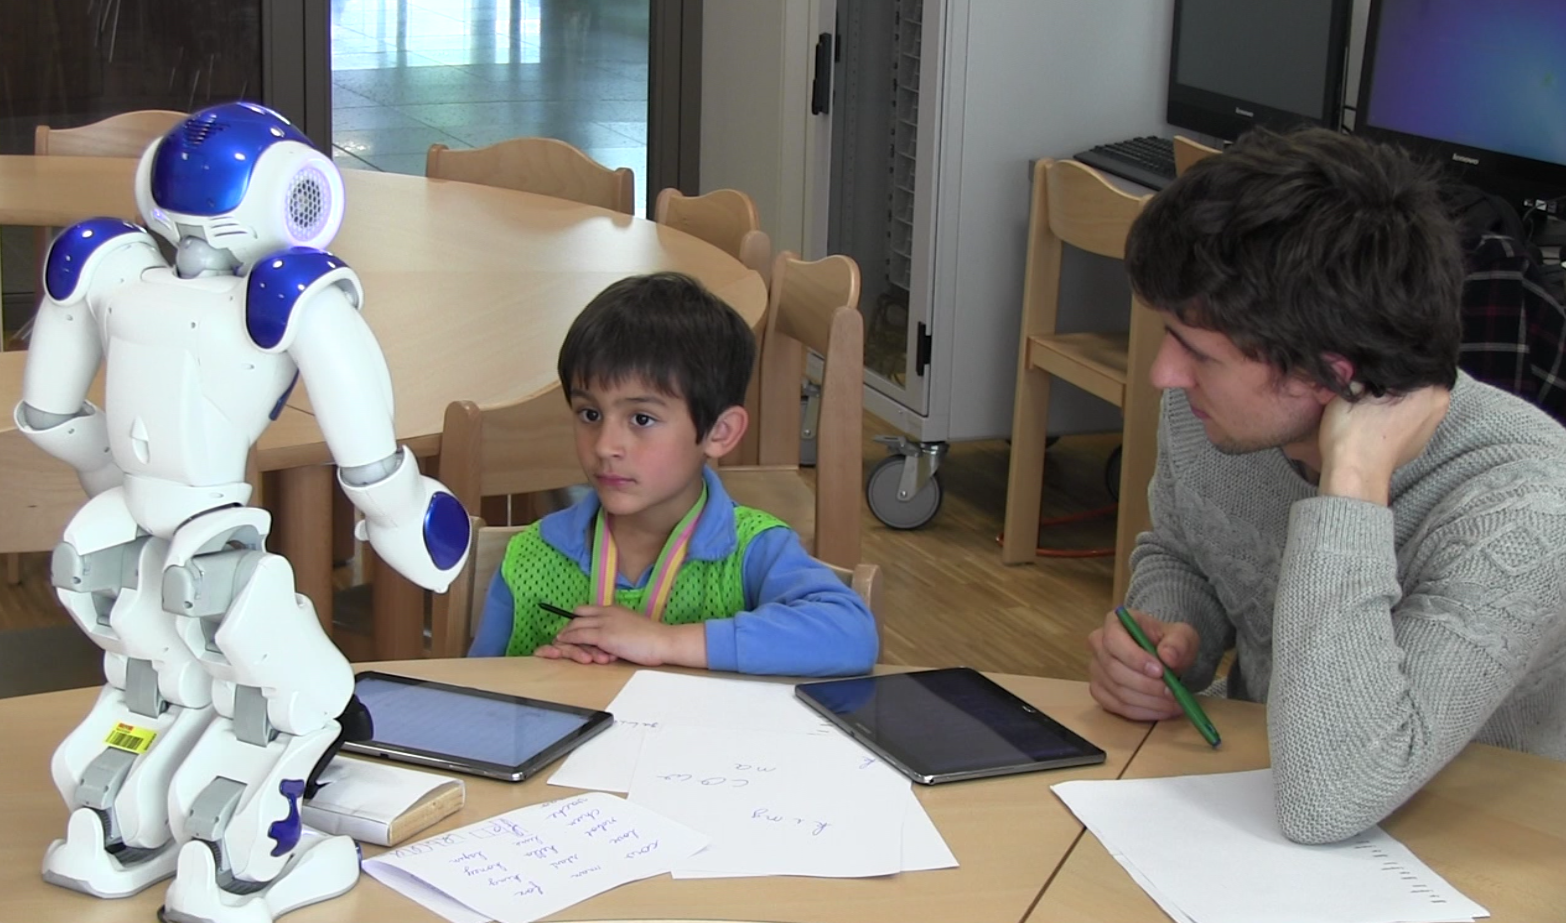
\includegraphics[width=0.6\columnwidth]{realSetup}
       \caption{\small Our experimental setup: face-to-face interaction with a {\sc
           nao} robot.  The robot writes on the tactile tablet, the child then
           corrects the robot by directly overwriting its letters on the tablet
           with a stylus. An adult (either a therapist or an experimenter,
           depending on the studies), remains next to the child to guide the work
           (prompting, turn taking, etc.). For some studies, a second tablet and an
           additional camera (to the feet of the robot) are employed.}

       \label{experimental_setup}
   \end{figure}
   
In \cite{jacq2016building}, we added buttons to the tablet interface to allow the child to evaluate the robot. Even if this feedback does not necessarily concerns the progress of the robot's writing (children also use them to express how they like the robot), we can still exploit and improve this idea to get effective information about the child's perception of the robot.
   
The robotic implementation of this activity is explained in \cite{Hood}. We used ROS to ensure the synchronization and communication between the different devices. Likewise, the cognitive architecture for mutual modelling will be deigned as ROS modules that will collect information about the mental state of agents (here, the child, or \textit{the robot-perceived-by-the-child}, or \textit{the child perceived by himself}) in order to update its model of these agents. Then, other modules (for example the module that governs the learning algorithm of the robot) will use these models to make decisions. We will better explain this design below, in sections \ref{framework} and \ref{arch}.

\subsection{Generating and learning letters}

Since our approach is based on teaching a robot how to write, generating (initially
bad) letters and learning from demonstration is a core aspect of the project.
The initial state of the robot and its ability to obviously learn from demonstrations of the child is the key to lend credibility to the activity and to induce the ``prot\'eg\'e" effect.

The technical idea is simple: allographs of letters are encoded as a sequence of 70 points in
2D-space and can be seen as vectors with 140 elements
($x_1,...,x_{70},\hspace{1mm}y_1,...,y_{70}$). We arbitrary chose a set of allograph
that define the initial state of generated letters. 
After the child provided a demonstration of a letter, the algorithm
generates a new letter corresponding to the middle point between the last state and the
demonstration. Details of this algorithm are presented in \cite{Hood} and improvements are tested in \cite{jacq2016building}.

However, to keep the child engaged, the robot must learn at the right rate, not too fast otherwise the kid will have
no opportunity for improving his skills and not too slow otherwise he may lose
trust in his ability to improve the robot' skills. And a learning curve just based on the middle point between last state and demonstration will be too fast for one child, and too slow for another one. 
We need to make the robot aware of the child's perception of its progress to take decision about its own learning curve. This awareness should be taken in account in our mutual modelling implementation, described in section~\ref{arch}. 

\subsection{Long-term studies}\label{long}
We tested the CoWriter activity in real pedagogical/therapeutic context with
children in difficulty over repeated long sessions (40-60 min). Through 3 different
case studies, we explored and refined experimental designs and algorithms in
order for the robot to adapt to the
troubles of each child and to promote their motivation and self-confidence. We report positive observations, suggesting commitment of children to help the
robot, and their comprehension that they were good enough to be teachers,
overcoming their initial low confidence with handwriting. We detail the measures and results of these studies in the following 3 subsections:
\paragraph{Case-study 1: Vincent}
\subparagraph{Context}
Vincent\footnote{The names of children have been changed.} is five year-old. At school, he has difficulties to learn writing, particularly with cursive letters. From our perspective, Vincent is shy and quiet. He suffers from poor self-confidence much more than any actual writing problem. The experiment was conducted without any therapist, in our laboratory. A parent was here to accompany the child, but did not intervene during interactions. The child's personality, conditions and state evaluation were reported by the parent.
\subparagraph{Hypothesis}
In the CoWriter activity the child should be engaged as the leader of the interaction. 
With this study we consider the problem of long-term interactions. We hypothesize that with an appealing scenario children can maintain motivation in interacting with the robot during a handwriting activity for an hour over 4 sessions.
\subparagraph{Methodology}
Our goal was to provide Vincent with
an environment that would enable him to sustain engagement over four one-hour sessions, 
one session per week. We decided to introduce a scenario to elicit a strong ``prot\'eg\'e effect" and such induce a stronger commitment. While the child came with low motivation in writing exercise for himself, our idea was to use this effect to promote a new extrinsic motivation: improving the letters in order to help the robot. Details of the experimental design are presented in~\cite{jacq2016building}.
\subparagraph{Measures \& Analysis}
We measured the commitment of the child with the number of demonstration he provided. We also measured the duration of sessions. During the two last sessions, we recorded the time taken by the child to write each demonstration. After the experiment we interviewed the parent of the child. She was asked if she observed any impact of our activity on the child.
We compared the number of demonstrations provided by Vincent along the 4 sessions (reported on Table~\ref{table:vincent_sess}) and we summed the time spend by the child to write demonstration during the 2 last sessions.
\begin{table}[!]
    \centering
    \caption{\footnotesize Number of demonstrations provided by Vincent over the four sessions.}
    \begin{tabular}{lccccc}
        \toprule
        Session & S1 & S2 & S3 & S4 & Total\\ 
        Number of demonstrations & 23 & 34 & 52 & 46 & 155\\ 
        \bottomrule

    \end{tabular}
    \label{table:vincent_sess}
\end{table}
\subparagraph{results}
Overall, Vincent provided 155 demonstrations to the robot. We can see in Table~\ref{table:vincent_sess} that the number of demonstrations provided by Vincent was globally increasing along sessions while the difficulty of the activity was also increasing. Interestingly, as the number of demonstration decreased from session 3 to session 4, the total time spend to write demonstrations stayed relatively constant: 41.6s in session 3 ($\thicksim$0.8s per letter) and 41.1s in session 4 ($\thicksim$0.89s per letter). A explanation of this result could be that since the difficulty was increasing the child spent more time to write his demonstrations. From the parent's perspective, Vincent was actually showing a new motivation in improving his handwriting. He took pleasure to work with the robot and to accomplish his teacher's mission. This represents a promising initial
result: we can effectively keep a child committed into the activity with the robot for a relatively long periods of time (about 4 hours).
The the ``prot\'eg\'e" effect was actually induced and the child felt responsible for the robot's learning.

\begin{figure}
    \centering
    \subfigure[Initial letter, generated by the robot]{
        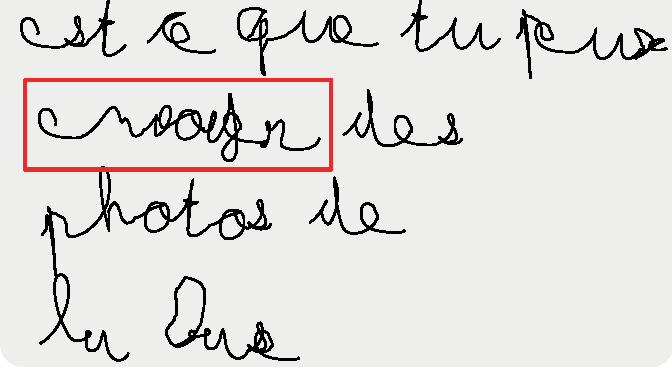
\includegraphics[height=3cm]{diego-initial-letter}
    }
    \subfigure[Final letter, after training with Vincent]{
        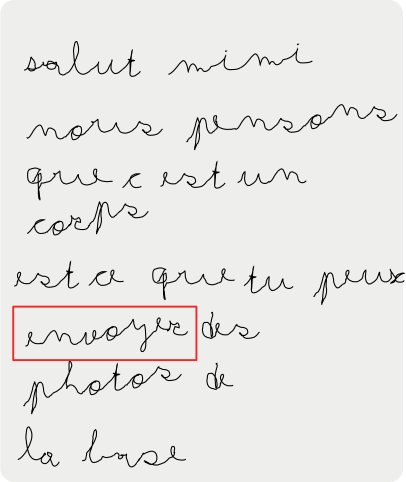
\includegraphics[height=3cm]{diego-final-letter}
    }

    \caption{\small (French) text generated by the robot, before and after a one
        hour long interaction session with the child. As an example, the red box
        highlights the changes on the word ``envoyer''.}

    \label{fig:stimuli}
\end{figure}

\paragraph{Case-study 2: Thomas}

\subparagraph{Context}
Thomas, five and a half years old boy, is under the care of an occupational
therapist. He has been diagnosed with visuo-constructive deficits.
He was frequently performing random attempts and then was comparing
with the provided template. According to the therapist, Thomas is restless and careless: he
rarely pays attention to
advice and does not take care of his drawing movement when he is writing. He is
quickly shifting his attention from one activity to another. Thomas was working on number allographs with his therapist. During a prior
meeting, the therapist provided us with a sequence of numbers
written by Thomas. One of the problems observed was drawing
horizontally-inverted allographs, mainly for ``5". The experiment was conducted with Thomas' therapist. 
\subparagraph{Hypothesis}
Our goal was to evaluate if the CoWriter activity could be adapted to a pedagogical context in order help a child with diagnosed deficits to learn handwriting. We believe that small modifications of the activity adapted to
Thomas' problems (visuo-constructive deficits and inattention) could help to
keep him focused on the activity during forty-minutes sessions, and to evidence to the child that the robot is progressing by dint of his demonstrations. 
\subparagraph{Methodology}
The experiment was conducted in the therapist's office (four sessions 
spanning over 5 weeks). We assumed that a scenario like the one we used 
for Vincent would not be usable with Thomas. We just introduced the robot 
and quickly said that it was seeking help to train for a robot handwriting contest. In order to integrate our work with that of the therapist, we decided to adapt the 
CoWriter activity to work with numbers. Details of the experimental design are presented in~\cite{jacq2016building}.
\subparagraph{Measures \& Analysis}
We recorded all the demonstration performed by the child and by the robot. The duration of sessions and the time spent by demonstration were also recorded by the logs of the tablet. It was difficult to make a comparison between different sessions since the child did not work on the same numbers. But we could study the evolution of the quality of Thomas' demonstration when he was working on a given number (Figure~\ref{Thomas_progress}).
To show how Thomas leaded the robot to reach his level we plotted on the same graph the evolution of the quality of Thomas' demonstrations and the robot's trials (Figure~\ref{Thomas_distances}). We also reconstructed and displayed the drawn allographs of the number 6 to visualize the impact of the lessons of Thomas on the robot (Figure~\ref{learning_6_demos}). 
\begin{figure}[!]
    \centering
    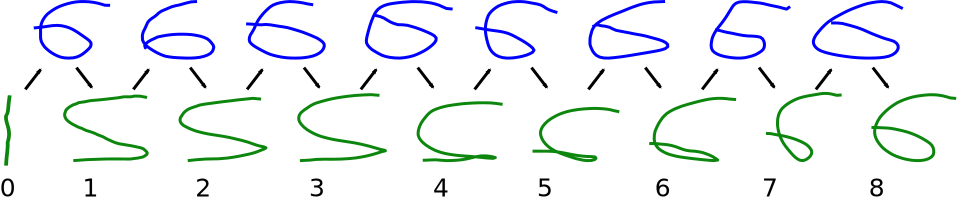
\includegraphics[width=0.6\linewidth]{learning_6_demos}
    \caption{\small Demonstrations provided by Thomas for the number ``6'' (top row) and
        corresponding shapes generated by the robot. After eight demonstrations,
        Thomas decided that the robot's ``6'' was good enough, and went to
    another character: in that respect, he was the one leading the learning
process of the robot.}
    \label{learning_6_demos}
\end{figure}
\subparagraph{Results}
Despite his attention deficit, Thomas was able to remain engaged in the activity during more than
forty minutes in each session. In total, 55 allographs out of 82 
demonstrated by the child were acceptable considering our threshold (with a
progressive improvement from 13 allographs out of 28 in the first session up to 26 out
of 29 in the last session).

\begin{figure}[!]
    \centering
    \subfigure[number 2]{
        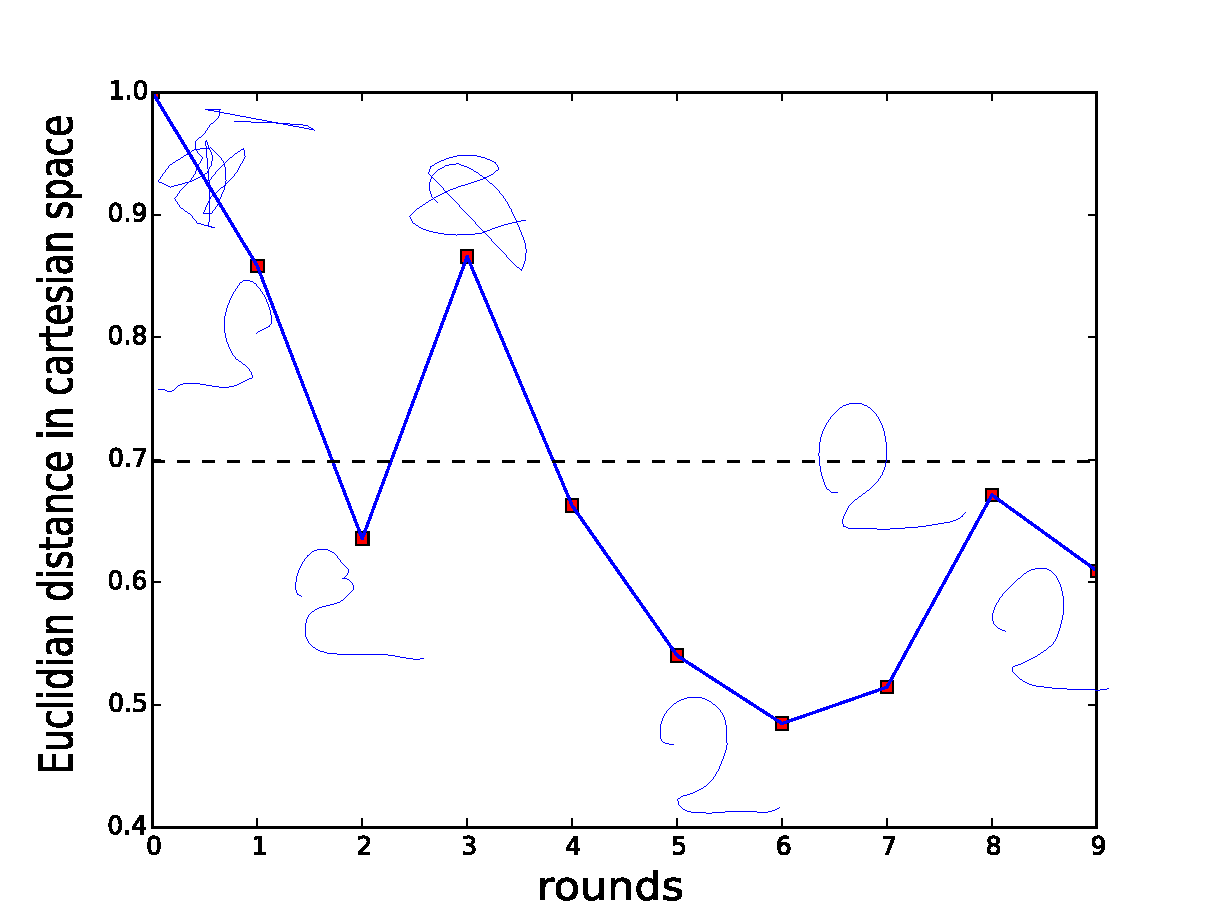
\includegraphics[width=5cm]{henry2}
    }
	\subfigure[number 5]{
        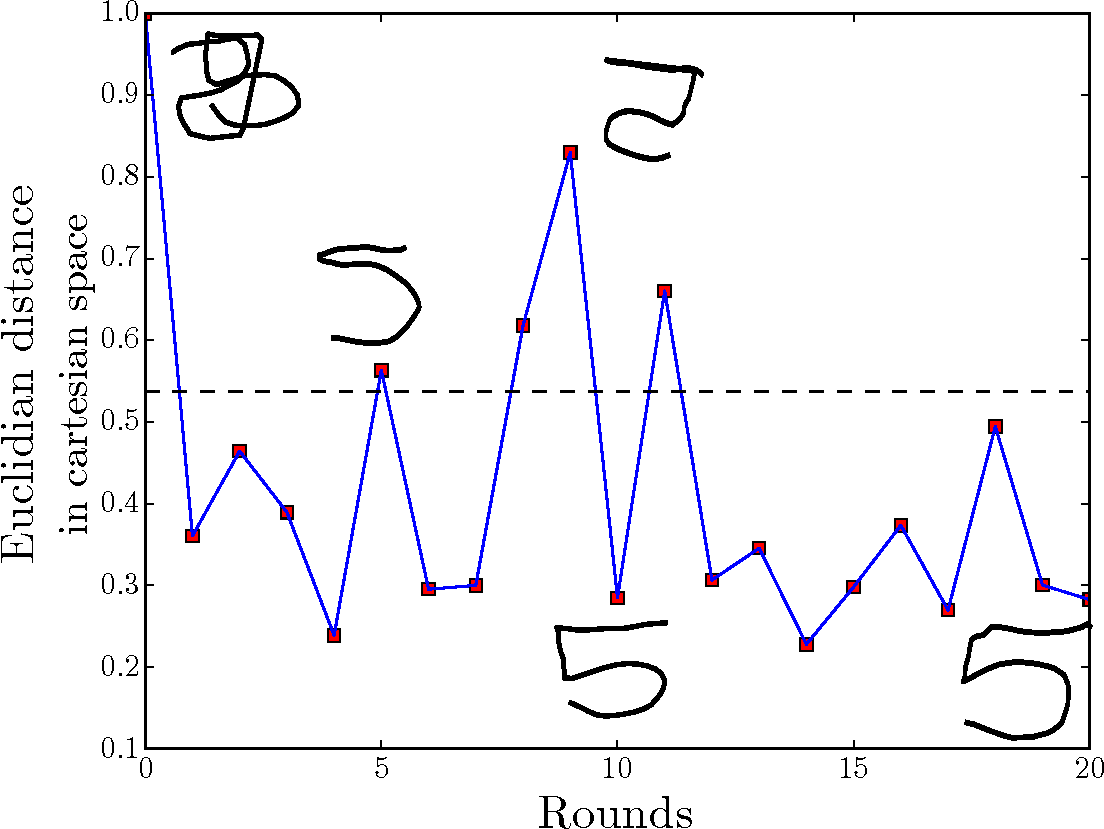
\includegraphics[width=5cm]{henry5}
    }
    \caption{\small Improvement of Thomas demonstrations for some numbers: a) the number 2 and b) the number 5. Thomas progressively took care of the demonstrations he was providing to the robot for those numbers. We used for this figure the same metric than the one used for the acceptance algorithm to measure distance between demonstration and templates. Distances are normalized with respect to the biggest value. The dashed line correspond to the threshold of robot's acceptance.}
    \label{Thomas_progress}
\end{figure}

As soon as Thomas understood that the robot was only accepting well-formed
allographs, he started to focus on it and he would typically draw 5 or 6 times
the number before actually sending to the robot (the tablet lets children
clear their drawing and try again before sending it). According to
the therapist, it was the first time that Thomas corrected himself in such a
way: he mad the effort to take into account how \emph{another agent} (the robot) would
interpret and understand his writing. Figure~\ref{Thomas_progress} shows how
he gradually improved his demonstrations for some numbers, according to the
metric we used to make the robot accept/refuse samples.

Since the robot's handwriting started from a simple primitive (a stroke), each
time Thomas succeeded to have his demonstrations accepted by it, the robot's
improvement was clearly visible (as measured in Figure~\ref{Thomas_distances}).
This led to a self-rewarding situation that effectively supported Thomas'
commitment.

\begin{figure}[!]
    \centering
    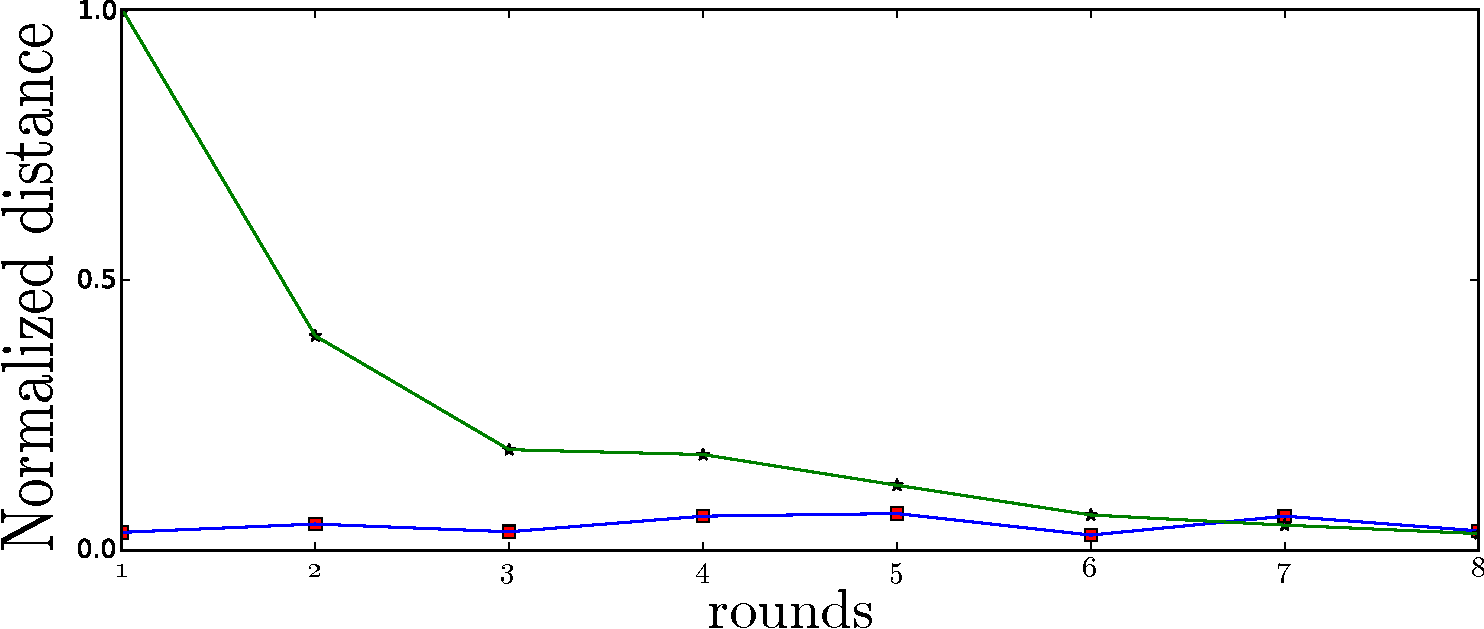
\includegraphics[width=0.5\linewidth]{learning_6_distances}
    \caption{\small Distance between demonstrations and templates. Green lines represent the robot performance,
blue lines performance of the child. The round IDs correspond to the demonstrations
pictured on Figure~\ref{learning_6_demos}.}
    \label{Thomas_distances}
\end{figure}


\paragraph{Clinic-study: when children evaluate the robot}
\subparagraph{Context}
Each of previous studies was specifically adapted to a particular child: we relied on two different
designs in order to sustain each child's commitment.
In this new experiment, we conducted a study with eight children using a single experimental design. The children all have in common difficulties to learn
cursive writing but the nature and magnitude of these troubles are significantly
different from one child to another. The experiment was conducted in collaboration with an occupational therapist. Our goal was to study the perception of the robot's progress in children. We wanted to know how easily children were able to take the role of teachers and to detect improvements or eventual degradations of the robot's letters.
\subparagraph{Hypothesis}
Children understand their role and find motivation to teach the robot. They are able to perceive the progress of the robot, and their evaluations correlates with its handwriting performance.
\subparagraph{Methodology}
This experiment took place in an occupational therapist clinic
in Normandy, France. Over a period of two weeks, each child came three times for a one hour long
session (except Adele and Marie who only attended one session). An experimenter was present to explain the rules of the game and tablet usage. As in the previous experiments, children were provided with two tablets: one to choose a word (or a single letter) to teach, one
used by both the child and the robot to write. We also provided printed templates for the letters if the child asked for them. 
Besides, we added two buttons to the tablet interface: a green one with a ``thumbs up", and
a red one with a ``thumbs down". Those buttons could be used by the children to evaluate the
robot (the green one was for positive feedback while the red one was for negative feedback). 
We used it as a measure of the perception of the robot by the child: the more the
child used evaluation buttons, the more he was adopting the role of the teacher, judging the
robot instead of himself. Children were free to use the buttons whenever they wanted during the experiment.
\subparagraph{Measures \& Analysis}
As in previous studies, we recorded the timestamps of all demonstrations, the duration of demonstrations and we measured the overall commitment of the children as the number of demonstrations provided per session. 
We also logged all the evaluations provided by the children. The awareness of children for the robot progress is measured as the correlation between children evaluations and distances between the robot's letters and reference templates.
Since sessions took place over only two weeks, we did not attempt to study possible
handwriting remediation in children, and we focused instead on the correlation between the children's evaluations and the robot's progression.
We estimated the robot's progression as the difference between an initial score
(score of the first robot's attempt when the children have chosen a new word/letter to
work on) and the current robot's score (after being taught by the child). The
score is calculated as the average of the euclidean
distance between the robot's generated letter and the reference allograph for each of the letters of the
word. The reference letters where manually created beforehand, based on typical cursive letters template\footnote{\url{http://www.education.com/slideshow/cursive-handwriting-z/}}. At every turn, we associate two values: the current score of the robot, and the child's immediate feedback (+1 if the child pressed the green button, -1 if he pressed the red one, 0 if he did not press any button during the round). We only keep rounds with feedback (\ie a non-zero grade) and computed a Pearson's correlation between the robot score and the child feedback.
\subparagraph{Results}
All children maintained their engagement during all the sessions. They provided
on average 42 demonstrations per session. All children made use of the evaluation buttons and
had preference to reward the robot (in total, 99 positive feedbacks and 33 negative ones were recorded). Interestingly, the time spent by the children to draw the demonstrations systematically increased from one session to the other. We interpret this result as the children being more careful and demonstrating the correct gestures to the robot in a slower fashion.

We found that five children out of the eight provided evaluations that significantly correlated with progress of the robot. The coefficients of correlation $r_{robot}$ are reported in Table~\ref{table:scores}.

We also computed the correlation between the children's evaluations and their own
progress. The analysis was conducted in the same way, using distances between the children's demonstrations and reference allographs as a progress score.
The evaluations of three out of the five children whose evaluations correlated with the robot's progress, were also significantly correlated with their own progress ($r_{child}$ in Table~\ref{table:scores}). For
those children, it seems that the robot was reflecting their own performances, and while they
were judging the robot positively (three times more positive feedback than negative feedback),
they were actually evaluating themselves.


\begin{table}
    \centering
    \caption{\footnotesize Feedback from the children to the robot. \emph{\#Demo}
        denotes the average number of demonstrations per session provided by the child;
        \emph{\#Pos} and \emph{\#Neg} the total number of positive (resp.
        negative) feedbacks they provided. $r$ (robot) is the correlation coefficient
        between the feedback provided by the children and the performance of the
        robot. $r$ (child) is the correlation coefficient
        between the feedback provided by the children and their own progress.
        }
    \begin{tabular}{ccccll}
        \toprule
        \bf Child      & \bf \# Demo & \bf \# Pos & \bf \# Neg & $r_{robot}$ & $r_{child}$ \\ \midrule
        \emph{Val\'erie} & 42           & 24              & 6               & 0.25 \small\tt ** & 0.14 \small\it ns\\ 
        \emph{\'Emilien} & 74           & 20              & 9               & 0.06 \small\it ns & 0.02 \small\it ns\\
        \emph{Mathieu} & 43           & 10              & 3               & 0.23 \small\tt ** & 0.21 \small\tt **\\
        \emph{Nicolas} & 38           & 16              & 4               & 0.31 \small\tt *** & 0.20 \small\tt **\\
        \emph{Johan}   & 32           & 10              & 5               & 0.10 \small\it ns & 0.03 \small\it ns\\
        \emph{Antoine} & 27           & 10              & 3               & 0.20 \small\tt * & -0.02 \small\it ns \\
        \emph{Ad\`ele}   & 35           & 4               & 2               & 0.28 \small\tt * & 0.30 \small\tt ** \\
        \emph{Marie}   & 40           & 5               & 1               & -0.02 \small\it ns & 0.13 \small\it ns\\ \bottomrule
    \end{tabular}

    \label{table:scores}
\end{table}


\subsection{With-me-ness}\label{with}
\emph{With-me-ness}, a concept borrowed from the
field of {\it Computer-Supported Collaborative Learning}, measures in a
well-defined way to what extent the human is \emph{with} the robot over the
course of an interactive task. As such, it is a meaningful precursor of
engagement. 
\paragraph{Description}
We explored a methodology, from real-time
estimation of the human's focus of attention (relying on a novel, open-source,
vision-based head pose estimator), to on-line computation of with-me-ness. The process can be described in 3 main steps (work published in~\cite{lemaignan2016realtime}):

\subparagraph{Head-pose estimation}
We derive the visual field of attention from the head pose. Our
technique only involves a single monocular RGB camera used for facial feature
extraction, and a static simplified 3D mesh of a human head.  68 facial features
are extracted using a fast template-based face alignment algorithm by Kazemi and
Sullivan~\cite{kazemi2014one}, as implemented in the open-source {\tt dlib}
library~\cite{dlib09}.  Eight of these features (chosen to be far apart and
relatively stable across age and gender) are then matched to their 3D
counterparts and we rely on an iterative $PnP$
algorithm (OpenCV's implementation) to compute the translation and rotation of
the head with respect to the camera frame. With this approach, knowing the
intrinsic parameters of the camera (calibrated camera) is required for an
accurate estimation of the absolute 3D localization of the head.

\subparagraph{Field and focus of attention estimation}
We model the field of attention as the central region of the field of view.  The
field of view itself is approximated to a cone spanned from the nasal depression
(sellion) of the human face. Different dimensions for the human field of view
can be found in the literature: Holmqvist~\cite{holmqvist2011eye} models it
with an horizontal aperture of $ \pm 40\degree $ and a vertical aperture of $
\pm 25\degree $, while Walker~\cite{walker1980clinical} for instance suggests
$60\degree$ up, $75\degree$ down, $60\degree$ inwards (towards the nose) and
$95\degree$ outwards.  Previous work on visual perspective taking for social
robotics~\cite{sisbot2011situation} model the field of attention as a cone of
$30\degree$. We retained in this work a slightly wider aperture of $40\degree$.
We then approximate the visual \emph{focus} of attention (VFoA) of the human to
the objects which lie inside this field of attention. At
a given time, more than one object can therefore be \emph{in focus}.

\subparagraph{Computing with-me-ness}
The concept of \emph{with-me-ness} has been introduced in the field of
\emph{Computer Supported Collaborative Learning} (CSCL) by Sharma~\etal
in~\cite{sharma2014me}. Sharma~\etal introduce this concept in an attempt to
answer a recurrent teacher's question: {\it ``how much are the students with
me?''}. They distinguish what they call \emph{perceptual with-me-ness} (the
student follows what the teacher refers to with deictic gestures) from
\emph{conceptual with-me-ness} (the student follows what the teacher refers to
verbally), and they show in an eye-tracking study that \emph{conceptual
with-me-ness} in particular correlates with better learning performance. This
also relates to the concept of gaze cross-recurrence that has been shown to
reflect the quality of the interaction~\cite{jermann2012effects} in
collaborative learning tasks. Sharma~\etal simply define \emph{conceptual with-me-ness} as the normalized
percentage of time during which the student's gaze overlapped the areas of
teaching slides currently referred to by the teacher.  In order to apply it to
human-robot interactions, we propose to extend this concept, and to define
\emph{conceptual with-me-ness} as the normalized ratio of time that the human
interactant focuses its attention on the attentional target expected by the
robot for the current task (or sub-task).
\paragraph{Validation}
We validated this approach with an experiment involving the CoWriter activity in a school.
The robot
controller would associate a set of expected attentional targets to the phase of
the interaction. For instance, while the robot was
waiting for the child's handwriting demonstration (``\textit{Waiting for
feedback}'' phase), the expected attentional target of the child was the tablet (since
the child was supposed to write there) or the secondary tablet (that displayed a
template of the word, used as a reference by the child). These expected targets
(green lines on Figure~\ref{fig:with-me-ness}) form the robot's attentional {\it
a priori} knowledge and are used to compute the with-me-ness. The with-me-ness plotted at the bottom of Figure~\ref{fig:with-me-ness} is computed on a sliding window of 30 seconds, and thus gives a picture of
``how well the child is following the robot's expectations'' at that time. As
seen, the with-me-ness computed at run-time by the robot (blue line) is
generally lower than the ground-truth (orange line, based on video-annotations),
and sometimes quite off, such as during episode marked ``A'': during that phase,
one can notice that the attention is mostly directed to undefined target {\sf
Other}, likely a consequence of inaccurate head detection.  

\begin{figure*}
    \centering
    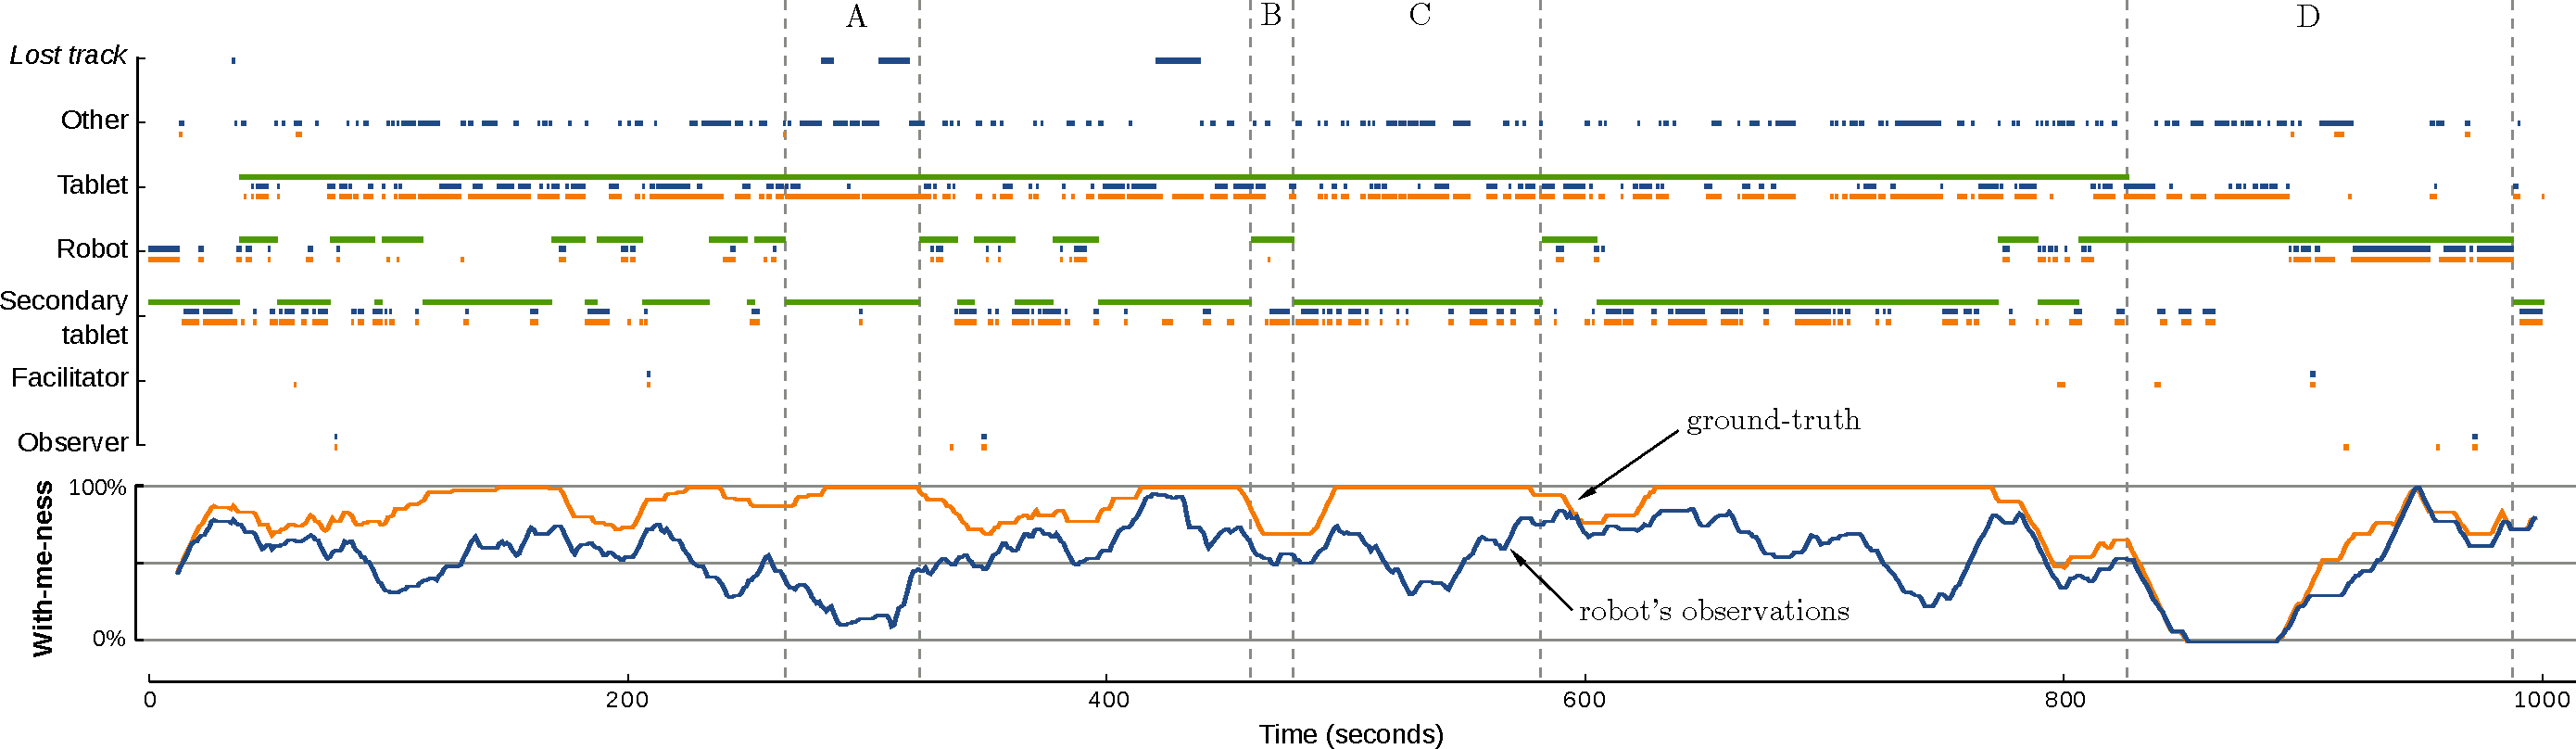
\includegraphics[width=\linewidth]{with-me-ness}
    \caption{\small \textbf{With-me-ness}. Evolution of the level of
        \emph{with-me-ness} over the whole $\approx$17min long interaction of
        the child. The bottom
        diagram represents the instantaneous level of with-me-ness over a
        sliding window of 30 seconds. The blue line is the with-me-ness as estimated
        by the robot, the orange line is the with-me-ness computed from manually
        annotated attentional targets.  Pearson's correlation between both
        series for this subject: $r(973)=0.58, p < .001$.}

    \label{fig:with-me-ness}
\end{figure*}

\subsection{Importance of these results in future works}
The CoWriter activity provides rich interactions, mostly non-verbal, full of misunderstandings between the child and the robot. For many reasons:
\begin{itemize}

\item The learning curve of the robot is often not adapted to the child's expectations (the robot is to slow to learn a word while the child is providing high number of perfect demonstrations or conversely too fast)
\item Most of the time the robot does not look at what the child wants him to look at or, contrariwise, the child is not looking what he is expected to look at (the last can be detected by the with-me-ness module presented above). 
\item When the child does a mistake (pushing a wrong button on the tablet or writing wrong letters as a demonstration) the robot could detect it and react in consequence.
\item Sometimes the child starts to be completely disengaged and the robot should react (by trying to call back the commitment of the child or by asking to stop the activity by itself).
\item The robot should wait to have the attention of the child in order to make sure that its trial of writing is being observed.
\item The robot should react as a student, but as a \textit{pretending} student in a didactic activity: if the child provides good feedback but is teaching a very wrong writing to the robot, the robot should be able to detect this situation and to say he does not want to learn this style. 

\end{itemize}
All those situations require a second level of mutual modelling to be solved by an unique reasoning.
The goal of my thesis is to build a cognitive architecture based on reasoning in two orders of mutual modelling. This architecture is expected to be generalizable and usable in different activities. But in order to make sure that this ability bring an improvement to HRI, it needs experimental evaluation involving  and interactive robot. 
This interaction must be studied over long-term sessions in order to facilitate the grounding of non-verbal mutual understandings, and to promote occurrences of misunderstanding situations. 
With the first case-study, we proved that the CoWriter activity is sustainable by one child over (at least) four sessions of one hour. 
The second case-study was to show that the activity can be used in real therapeutic context and could be an help for therapists: by improving this activity, a mutual modelling architecture could have a direct utility both in education and occupational therapy. 
The buttons for feedback tested by the clinic-study and the evaluation and calibration of the with-me-ness data will be a useful feature for mutual modelling. 
In the clinic-study, we saw that children could give coherent feedbacks to the robot which is a strong information about their perception of a robot as a student while they are the teachers. 
The VFoA tracker
%todo VFoA: abbrevations should be introduced with full form before being used
 will be used to keep a robust knowledge of what the child has seen and is looking at. This knowledge is essential to reason with 1st and 2nd level of mutual modelling. Furthermore, we believe that the interaction could be improved by adding some micro-behaviours to the robot (short gazes or arm's gestures, non-verbal language) that such abilities.

\section{Framework for mutual modelling in robotics}\label{framework}
\subsection{Justification of the approach}

A first intuition for mutual modelling (MM) is to assume that all agents have the same architecture. In~\cite{breazeal2006using}, Breazeal shows a MM-based reasoning where the robot uses its own architecture to model other agents. We can imagine a second level of modelling where the robot recursively attribute to other agents the mutual modelling ability. But that can create an infinite recursive loop: the agent then models the robot that models the agent etc. Another reasons to avoid an infinite recursive approach is that different agents must have different behaviours: in similar situations, they do not necessary take similar decisions. 

We propose a different approach of modelling, where we define two orders of agent's model: the \textbf{first-order-agents} concern direct representations of agents by the robot (for example the child), while the \textbf{second-order-agents} concern the representation of agents by agents (for example the robot-perceived-by-the-child). 
Modelling second-order-agent like the robot-perceived-by-the-child, helps to model how the child perceives the robot, e.g. to make sure the child understand that the robot is learning from his demonstrations. 
We can as well define $\textbf{n}^{\textbf{th}}$\textbf{-order-agents} with a higher level of theory of mind. But taking into account high levels of mutual modelling would be difficult to process in real time. Unlike the epistemic logic, our proposed framework will not take into account infinite regress~\cite{clark1991grounding} of mutual modelling.

\subsection{Notations}\label{not}
$M_R\left[\textit{A}\right]$ stands for \textcolor{wine}{the model (built by the robot R) about the agent A} (first-order-agent). $M_R\left[\textit{A,B}\right]$ stands for \textcolor{wine}{the model (built by the robot R) about the agent B perceived by the agent A} (second-order-agent). 
As said above, we limit our approach to 1st and 2nd order of modelling. In a two-agents interaction (the child and the robot) we will focus on three models: $ M_R\left[\textit{C}\right]$ (the model about the child), $ M_R\left[\textit{R}\right]$ (the model about the robot) and $ M_R\left[\textit{C,R}\right]$ (the robot perceived by the child). 
It would be also interesting to study $ M_R\left[\textit{C,C}\right]$, the model about the child perceived by himself in order to play with his self-confidence. But detecting differences between $ M_R\left[\textit{C}\right]$ and $ M_R\left[\textit{C,C}\right]$ seems difficult with the current abilities of the robot. 

As models are dynamic, $ M^t_R\left[\textit{A}\right]$ represent the model about an agent A at time $t$.

\subsection{Mutual understanding}
Given those three models ($ M_R\left[\textit{R}\right]$, $ M_R\left[\textit{C}\right]$ and $ M_R\left[\textit{C,R}\right]$) the robot must be able to detect misunderstandings. 
A misunderstanding of an agent $A$ by the robot can be formalised as a error between what is actually in the mind of the agent (we can call it $\Phi[A]$) and the model built by the robot: $\Delta \left(\Phi[A] ; M_R\left[\textit{A}\right]\right)$. But if $A$ is human, $\Phi[A]$ is inaccessible to the robot. In order to maintain a mutual understanding, humans~\cite{suzuki2015neural} (and monkeys~\cite{haroush2015neuronal}), use predictions of others' behaviours. A bio-inspired approach would be to make, at time $t$, a prediction $P^{t+1}_R\left[\textit{A}\right]$ of the model. Then, at time $t+1$, the robot can compute a \textbf{prediction error} $\Delta \left( M^{t+1}_R\left[\textit{A}\right]; P^{t+1}_R\left[\textit{A}\right]\right)$ in order to detect such a misunderstanding. This idea rely on the assumption that the better are the predictions of a model, the better the model fits the reality. Then, the dynamic of the model can be updated according to the resulting error of prediction. This rule can be used with $ M_R\left[\textit{C}\right]$ and $ M_R\left[\textit{C,R}\right]$. 

Another type of misunderstanding concerns the comprehension of the robot by the child: using the same formalism, it is an error between the actual perception of the robot by the child (we can call it $\Phi[C,R]$) and the robot itself: $\Delta \left(\Phi[C,R] ; M_R\left[\textit{R}\right]\right)$. Again, the robot does not have access to $\Phi[C,R]$, but it approximates it with $ M_R\left[\textit{C,R}\right]$. Finally we define the \textbf{child's perception error} at time $t$ by $\Delta \left(M^t_R\left[\textit{C,R}\right] ; M^t_R\left[\textit{R}\right]\right)$. This error is taken in account only if the robot has a correct model of itself perceived by the child (only if $M_R\left[\textit{C,R}\right]$ produce small prediction errors). Since this error assumes that models built by the robot are correct, it is not used to update these models. It corresponds to an error of the child: in order to repair it, the robot must explain the misunderstanding to the child or exaggerate an action to make sure it will be understood.

As an example, in the CoWriter activity, the child teach handwriting to the robot. The robot pretends to be a beginner, but it has its idea of a good handwriting. The robot is perfectly aware of its played progresses. But we want the child to be aware of the progress of the robot. In that perspective, the child's perception error corresponds to the sentence ``\textit{I make progress but the child think I don't}", while the prediction error of $M_R\left[\textit{C,R}\right]$ corresponds to ``\textit{The child think I don't make progress, but maybe he think I do and I haven't understood him}".  

\subsection{Structure and dynamic of the models}
Each model contains the knowledge, mental states and possible actions of an agent. The dynamic between actions and knowledges must be encoded. Some causality can be assumed in advance (if the child gives a good feedback to the robot, it means that the robot-perceived-by-the-child makes progresses) while other can be learnt (e.g. if each time the robot looks at the head of the child, the child stops to write). Each modelled agent has its own goals, encoded as a reinforcement learning process. As an example, in CoWriter the robot-perceived-by-the-child ($ M_R\left[\textit{C,R}\right]$) is a learner and has the simple goal to make progress. The child ($ M_R\left[\textit{C}\right]$) is modelled as a teacher and is assumed to have the goal to improve the robot's writing. Then, the goal of the robot ($ M_R\left[\textit{R}\right]$) is to keep a mutual understanding: its knowledges and actions must correspond to itself perceived by the child, and it must be able to predict the behaviour of the child. The Figure~\ref{mm} visually summarizes this example.

The goals of $ M_R\left[\textit{C}\right]$ and $ M_R\left[\textit{C,R}\right]$ depend on the activity and must be programmed each time we move to a new activity. They can be improved to better fit the child's behaviour by learning from experience. Contrariwise, the goal of $ M_R\left[\textit{R}\right]$ to keep a mutual understanding is independent and reusable. 

All sensors (cameras, micros, motor positions etc. and in the case of CoWriter the tablet's inputs) are used to perceive information about the physical behaviour of agents. 
We call all the measurable quantities or qualities that provide information like position in space, the direction of the gaze, speech, movement and facial expressions etc. as \textit{perceived variables}. 
Each agent's model is associated with a set of perceived variables that describes his physical behaviour (mostly actions).

Knowledge and emotional states of agents cannot be directly measured by the  sensors. 
We call \textit{abstract variables} all the quantities or qualities that describe the mental state of an agent. 
Abstract variables are deduced from the dynamic of perceived variables. 
As an example, if the robot points at an object with its arm, it expects the child to look at the object. 
If then the child looks at the hand of the robot, the robot can deduce that the child has not understood the meaning of its gesture. 
The perceived variables are the robot's gesture and the gaze direction of the child. 
The deduced abstract variable is the understanding of the gesture by the child. 


\begin{figure}[!]
\centering
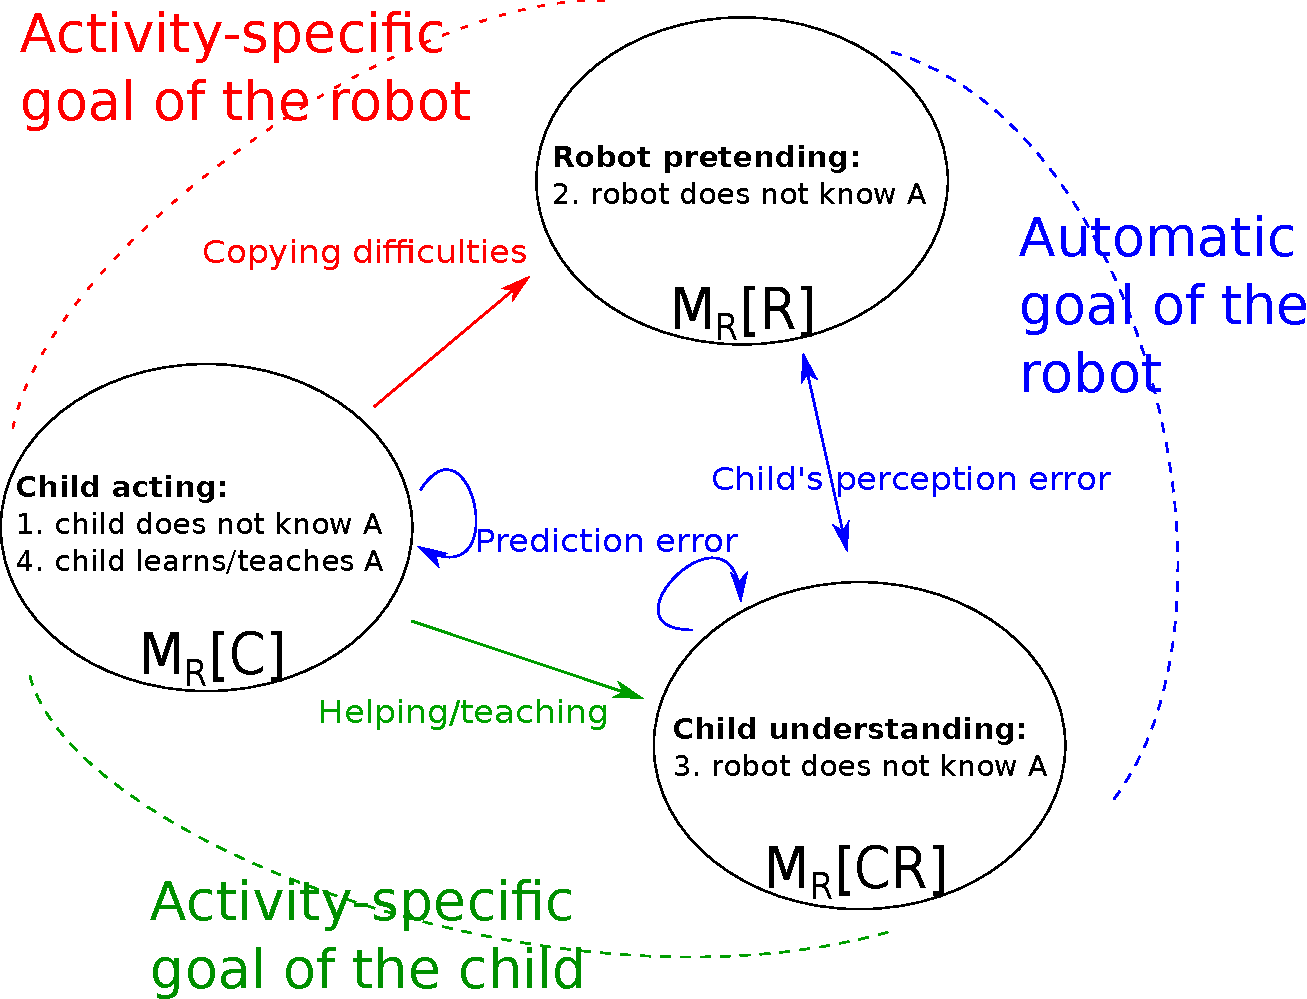
\includegraphics[width=0.6\columnwidth]{mutual_behaviour}
\caption{\small The different goals of agents and their behaviours in the perspective of our framework. We present a generic example where the child learns by teaching a knowledge A, that could represent the allograph of a letter. In the case of the CoWriter activity, the goal is to copy and exaggerate the errors of the child in order to induce a ``prot\'eg\'e" effect (red arrow) and we expect that the child will find motivation to teach the robot if we successfully induce this effect (green arrow). The robot uses predictions of $ M_R\left[\textit{C}\right]$ and $ M_R\left[\textit{C,R}\right]$ and coherence between $ M_R\left[\textit{R}\right]$ and $ M_R\left[\textit{C,R}\right]$ in order to detect different kind of misunderstandings (blue arrows).}
\label{mm}
\end{figure} 

\section{Implementation}\label{arch} 

\subsection{Perception}
\label{ssec:perception}
Sensitive modules produce values of relevant perceived variables from various sensors. 
While the agent's gaze direction and facial expression can be used in any interaction, some additive variables can be specific to the activity: in CoWriter, a module uses the tablet's input (demonstration of writing of the child) to compute the new state of robot's writing. The level of writing of the child and the robot are encoded as perceived variables by the models of the robot and the child.
The evaluation of the robot by the child via the feedback buttons on the tablet defines another perceived variable provided by the modules of the activity. 
Other modules can be independent of the activity: the system that tracks the VFoA of the child and estimates the with-me-ness provides additive information not directly used by the modules of the activity.  

\subsection{Mutual models}
\label{ssec:mmm}
Each perceived value produced by the sensitive modules are associated with the model of an agent (or a $2^{th}$-order agent, like $M_R\left[CR\right]$). As an example, the VFoA of the child is associated to the model of the child, while the position of the head of the robot is a variable associated to the robot.
The model of the robot $M_R\left[R\right]$ and the robot viewed by the child $M_R\left[CR\right]$ must contain the same variables in order to be comparable. But they are not governed by the same dynamic.
A model encodes the values of perceived and abstract variables and their dynamics. Also, the dynamic of variables from one model to another one must be encoded (an action of the robot has an impact on the behaviour of the child and an action of the child, like a feedback, has an impact on $M_R\left[CR\right]$). Different approaches can be use in order to encode this dynamic (bayesian, hebbian network, reinforcement learning, mixtures hebbian+reinforcement...). This dynamic is both used to establish predictions and to take decisions.

\subsection{Decision making}
\label{ssec:decision}

As we said above, the robot has two goals: one being the maintenance of a mutual understanding, the second being the goal of the activity. 
In CoWriter, we want to build a ``prot\'eg\'e effect" in order to induce in the child an extrinsic motivation to practice handwriting. 
In that perspective, the behaviour of the robot is to pretend that its handwriting is so poor that the child should be convinced he can and must help the robot. Then, in order to maintain this effect, the robot must adopt a convincing behaviour as a student, making progress thanks to the demonstrations of the child. 

The only decision associated with the activity is to write with a handwriting style that will be convincing for the child. 
But the choice of this style and all other behaviours (robot's gaze direction, gestures, potential short speech) are made in order to maintain a mutual understanding. 
If the robot detects that it misunderstood the child (prediction error) it corrects the wrong dynamic of the models and, if it's important, it can tell the child about its mistake. 
If it detects that the child misunderstood the robot (child's perception error) it must repair the situation in order to be understood. 
An idea to figure out the good action (or sequence of actions) that leads to help the child to understand could be to inverse the causality dynamic to find what actions (or mental state) caused good understanding in $M_R\left[CR\right]$. 

An example of such process is the following: The robot uses a bad handwriting after a demonstration of the child. 
In $M_R\left[R\right]$, a variable representing the current level of handwriting takes a small value (0.1). Then, the child responds with a positive feedback. This positive feedback of the child leads to an higher value of the same variable in $M_R\left[CR\right]$ (0.7). As the difference between these variables is high (0.6), the robot wants to repair this misunderstanding. 
The process will look for what led to a small level of writing in $M_R\left[CR\right]$, that is a negative feedback of the child. Then, what leads to a negative feedback of the child is a very poor trial of writing of the robot and the fact that the child is looking at the tablet in the same time. Also, in order to conduce the child to look at the tablet, maybe the robot has to first look at the child waiting for an eyes-contact, then to look at the tablet. So the robot takes the decision to look at the child in the eyes, and then to look at the tablet. If the child follows this gesture and also looks at the tablet, the robot starts to write in a very bad style the same word (exaggerating the mistakes) and expect that this time the child will give a negative feedback.

Some decisions can have a high impact on the interaction: to stop an activity and to switch to a new one can frustrate a child that was committed. 
The conditions to make this decision are not directly assessable, but must be learned by the robot. In order to make these decisions cautiously, we propose to start with a Wizard-of-Oz approach and to move towards an autonomous approach following these steps: 
\begin{enumerate}
\item \textbf{Wizard-of-Oz}: A human takes decisions; the robot learns
\item \textbf{Mixed-initiative}: The robot makes suggestions; a human agrees or disagrees
\item \textbf{Autonomous}: The robot makes decisions
\end{enumerate}

% tetailler ce genre d'approche (surtout woz)

\subsection{ROS} % pas sur

The architecture will be implemented using ROS to synchronize the activity of the different parts of this architecture (written as ROS nodes). The perceived variables provided by sensitive modules and abstract variables provided by expected causalities will be published as messages on topics specific to the associated models. In the same way, decisions taken will be sent as messages to the robot's control and tablets application in order to be realized. 

\subsection{Integration to CoWriter}

The CoWriter activity is already implemented using ROS. The main nodes that provide values of relevant variables are the robot's state machine, the node that governs the algorithm to learn/generate letters and the interpreter of the tablet inputs. Variables are already published on other topics used for the dynamic of the activity. We will additionally publish them on the topics associated to the mutual modelling architecture. 

\section{Evaluation}\label{eval}

\subsection{Hypothesis}

The question of this thesis concerns the improvement of human-robot interaction brought by mutual modelling, especially in the educational context of the CoWriter activity. In order to evaluate this improvement, we hypothesize the following assertion:\\

%\begin{itemize}
\textit{- Decisions made via our architecture aiming to maintain mutual understanding, improve the quality of human-robot interaction.}\\
%\end{itemize}

Regarding our applicative context, the CoWriter project, we can develop this hypothesis into the following two sub-hypothesis:\\

%\begin{itemize}
\textit{- Our architecture improves the interaction in the CoWriter activity} (1).\\
\textit{- Our architecture is generalisable and can be adapted to other activities} (2).\\
%\end{itemize}

To study hypothesis (1), we need to rigorously define the \textit{quality of the interaction}.\\
Since the goal is to promote extrinsic motivation by inducing a ``prot\'eg\'e" effect, we would like to measure the motivation of the child to play the activity and his satisfaction of the robot's progress. As we justified in section~\ref{not}, we will not (at least in a first time) look at the improvement of children self-esteem, that is a second goal of CoWriter. 
%todo la phrase d'avant est pas clair. du coup quel sont tes mesures de quality of interaction? , il faut pointer vers la section d'apres
Hypothesis (2) will be verified by designing different interactions, not necessary related to an educational context, that will be based on tasks that need 2nd order of modelling and mutual understanding in order to be solved.
%todo donne un exmaple ou pointe vers un example
\subsection{Experimental studies}

In CoWriter, a measure of the quality of the interaction can be defined by several variables that provide cues about the commitment of the child (quantity of demonstrations, time spent to write demonstrations, quality/progress of demonstration, progress of the robot, \textit{with-me-ness} ...). The evaluation with feedback buttons can also be used to estimate how the child understands his role of teacher.

Some experiments will be conduced in order to develop the architecture and to test it step by step. 
As an example, we will start with a small number of variables (perceived variables that are ready like the VFoA, children's feedback and level of writing) and a small set of actions (gaze direction, style of writing) and we will conduct experiments in order to understand how to initialise the dynamics of those variables. 
Also, we will need to define how the robot should react when it exaggerates a bad handwriting. And we will progressively add new variables  and new actions to take into account. 
Each time we will test and parametrize the new improvements with experiments. Such experiments requires high number of children but does not require long-term studies. They will be conduced in schools as we did to setup and verify the with-me-ness in~\ref{with}.

When the architecture will be enough enriched with perceived/abstract variables and actions, we will figure out the possible improvement brought by the architecture and hence verify the hypothesis (1) via long-term studies. It will not necessary requires high number of children (may be 10 will be enough). One half of children will interact with the robot using mutual modelling reasoning and the other half (control group) will interact with the robot without mutual modelling (the current state of the activity). We will also verify the hypothesis (2) with group of children (or adults, depending on the activity) where only a half will interact with a mutual modelling robot. these last experiment will not requires long-term studies like with CoWriter, but maybe high number of subject will be required.

\section{Conclusion and planning}

We presented in this paper the research question of this thesis, which concerns the importance of mutual modelling in educative human-robot interactions. In order to study this question, we will develop an architecture based on mutual modelling that will collect information about mental and physical states of different agent. The stages of this construction will correspond to the successive additions of variables (or groups of variables) to take into account by the models. We will progressively extract pieces of response to our research question by testing our system each time a stage is crossed. We will use the framework for mutual modelling in HRI that we introduced in~\ref{framework} in order to simplify notations and clarify the concepts. 

\bibliographystyle{abbrv}
\small
\bibliography{biblio} 

\end{document}
